\documentclass{article}
\usepackage[utf8]{inputenc}
\usepackage{caption}
\usepackage{amsmath}
\usepackage{amssymb}
\usepackage{mathtools}
\usepackage{multicol}
\usepackage{graphicx}
\usepackage{wrapfig}
\usepackage{float}
\usepackage[makeroom]{cancel}
\usepackage{mhchem}
\usepackage{pst-plot}

\graphicspath{ {../images/} }

\renewcommand{\familydefault}{\sfdefault}
\renewcommand{\baselinestretch}{1.5} % line spacing
\newcommand{\fline}{\par\noindent\rule{\textwidth}{0.1pt}} % horizontal line (wide)

\title{Topic 8 Acids \& Bases\\Lesson 6 - Titration Reactions}
\author{Peter Zhang}

\begin{document}

\maketitle
\tableofcontents
\newpage

% lesson 
\section{Titration Reactions}
pH curves can be used to determine equilavence point\\halfway point once a vertical jump in pH accurs at specific values

\begin{enumerate}
\subsection{Strong and Strong Reactions}
\item Strong and Strong\\
Ex: If $50cm^3$ of 0.3M HCl is titrated with 0.3M NaOH, find:\\
a) Starting pH of acid
$$pH = -\log{(0.3)} = 0.52$$
b) pH after adding $25cm^3$ of base
\begin{figure}[H]
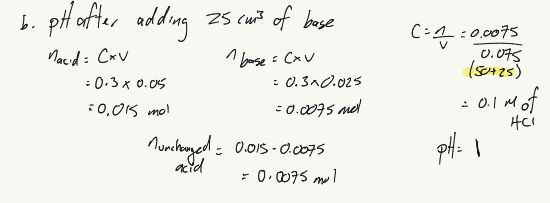
\includegraphics[width=\textwidth]{4.6fig1.png}
\captionof{figure}{Solution for b)}
\end{figure}

\begin{figure}[H]
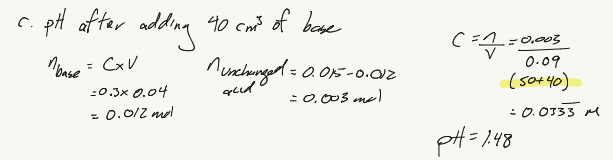
\includegraphics[width=\textwidth]{4.6fig2.png}
\captionof{figure}{Solution for c)}
\end{figure}

\begin{figure}[H]
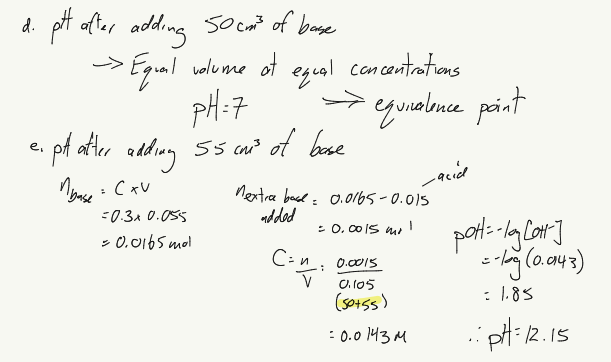
\includegraphics[width=\textwidth]{4.6fig3.png}
\captionof{figure}{Solutions for d) and e)}
\end{figure}

\subsection{Weak and Strong Reactions}
\item Weak and Strong\\
If weak acid pH overall will be greater than 7 at equivalence point\\If weak base pH will be less than 7.
\begin{itemize}
\item basically the stronger substance will determine the final value of the pH at the equivalence point
\item strong acid + weak base = acidic overall
\item weak acid + strong base = basic overall
\end{itemize}

\begin{itemize}
\item When mixing half the volume of the it gives half the equivalence point\\considered a buffering region (change is slow and gradual)
\item [acid] = [salt] (or [base] = [salt])
\item so $\rightarrow$ [acid] = [HA] + [salt]
\item and [HA] = [A-]
\item $\therefore K_{a} = \ce{[H+]}$ and $pK_{a} = pH$
\end{itemize}

\begin{figure}
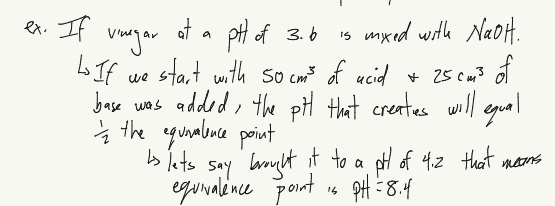
\includegraphics[width=\textwidth]{4.6fig4.png}
\captionof{figure}{Solving for a reaction between vinegar (weak acid) and NaOH (strong base)}
\end{figure}


\end{enumerate}
\subsection{Weak + Weak}
\textbf{NO CALCULATIONS DUE TO MINIMAL CHANGE IN CONCENTRATION OF REACTANTS AND PRODUCTS}












\end{document}